\section{biguint-div}
\label{biguint-div}

Note that div-rem has the same constraints logic with div

\begin{enumerate}
    \item target
        \begin{itemize}
            \item implement the division of two biguints
        \end{itemize}
    \item constraints-logic
        \begin{itemize}
            \item not implement div-algrithem directly
            \item use nondeterministic feature to check div-logic
            \item check div * b + rem = a
            \item check rem < b
        \end{itemize}
    \item div-process layout
        \begin{figure}[!ht]
            \centering
            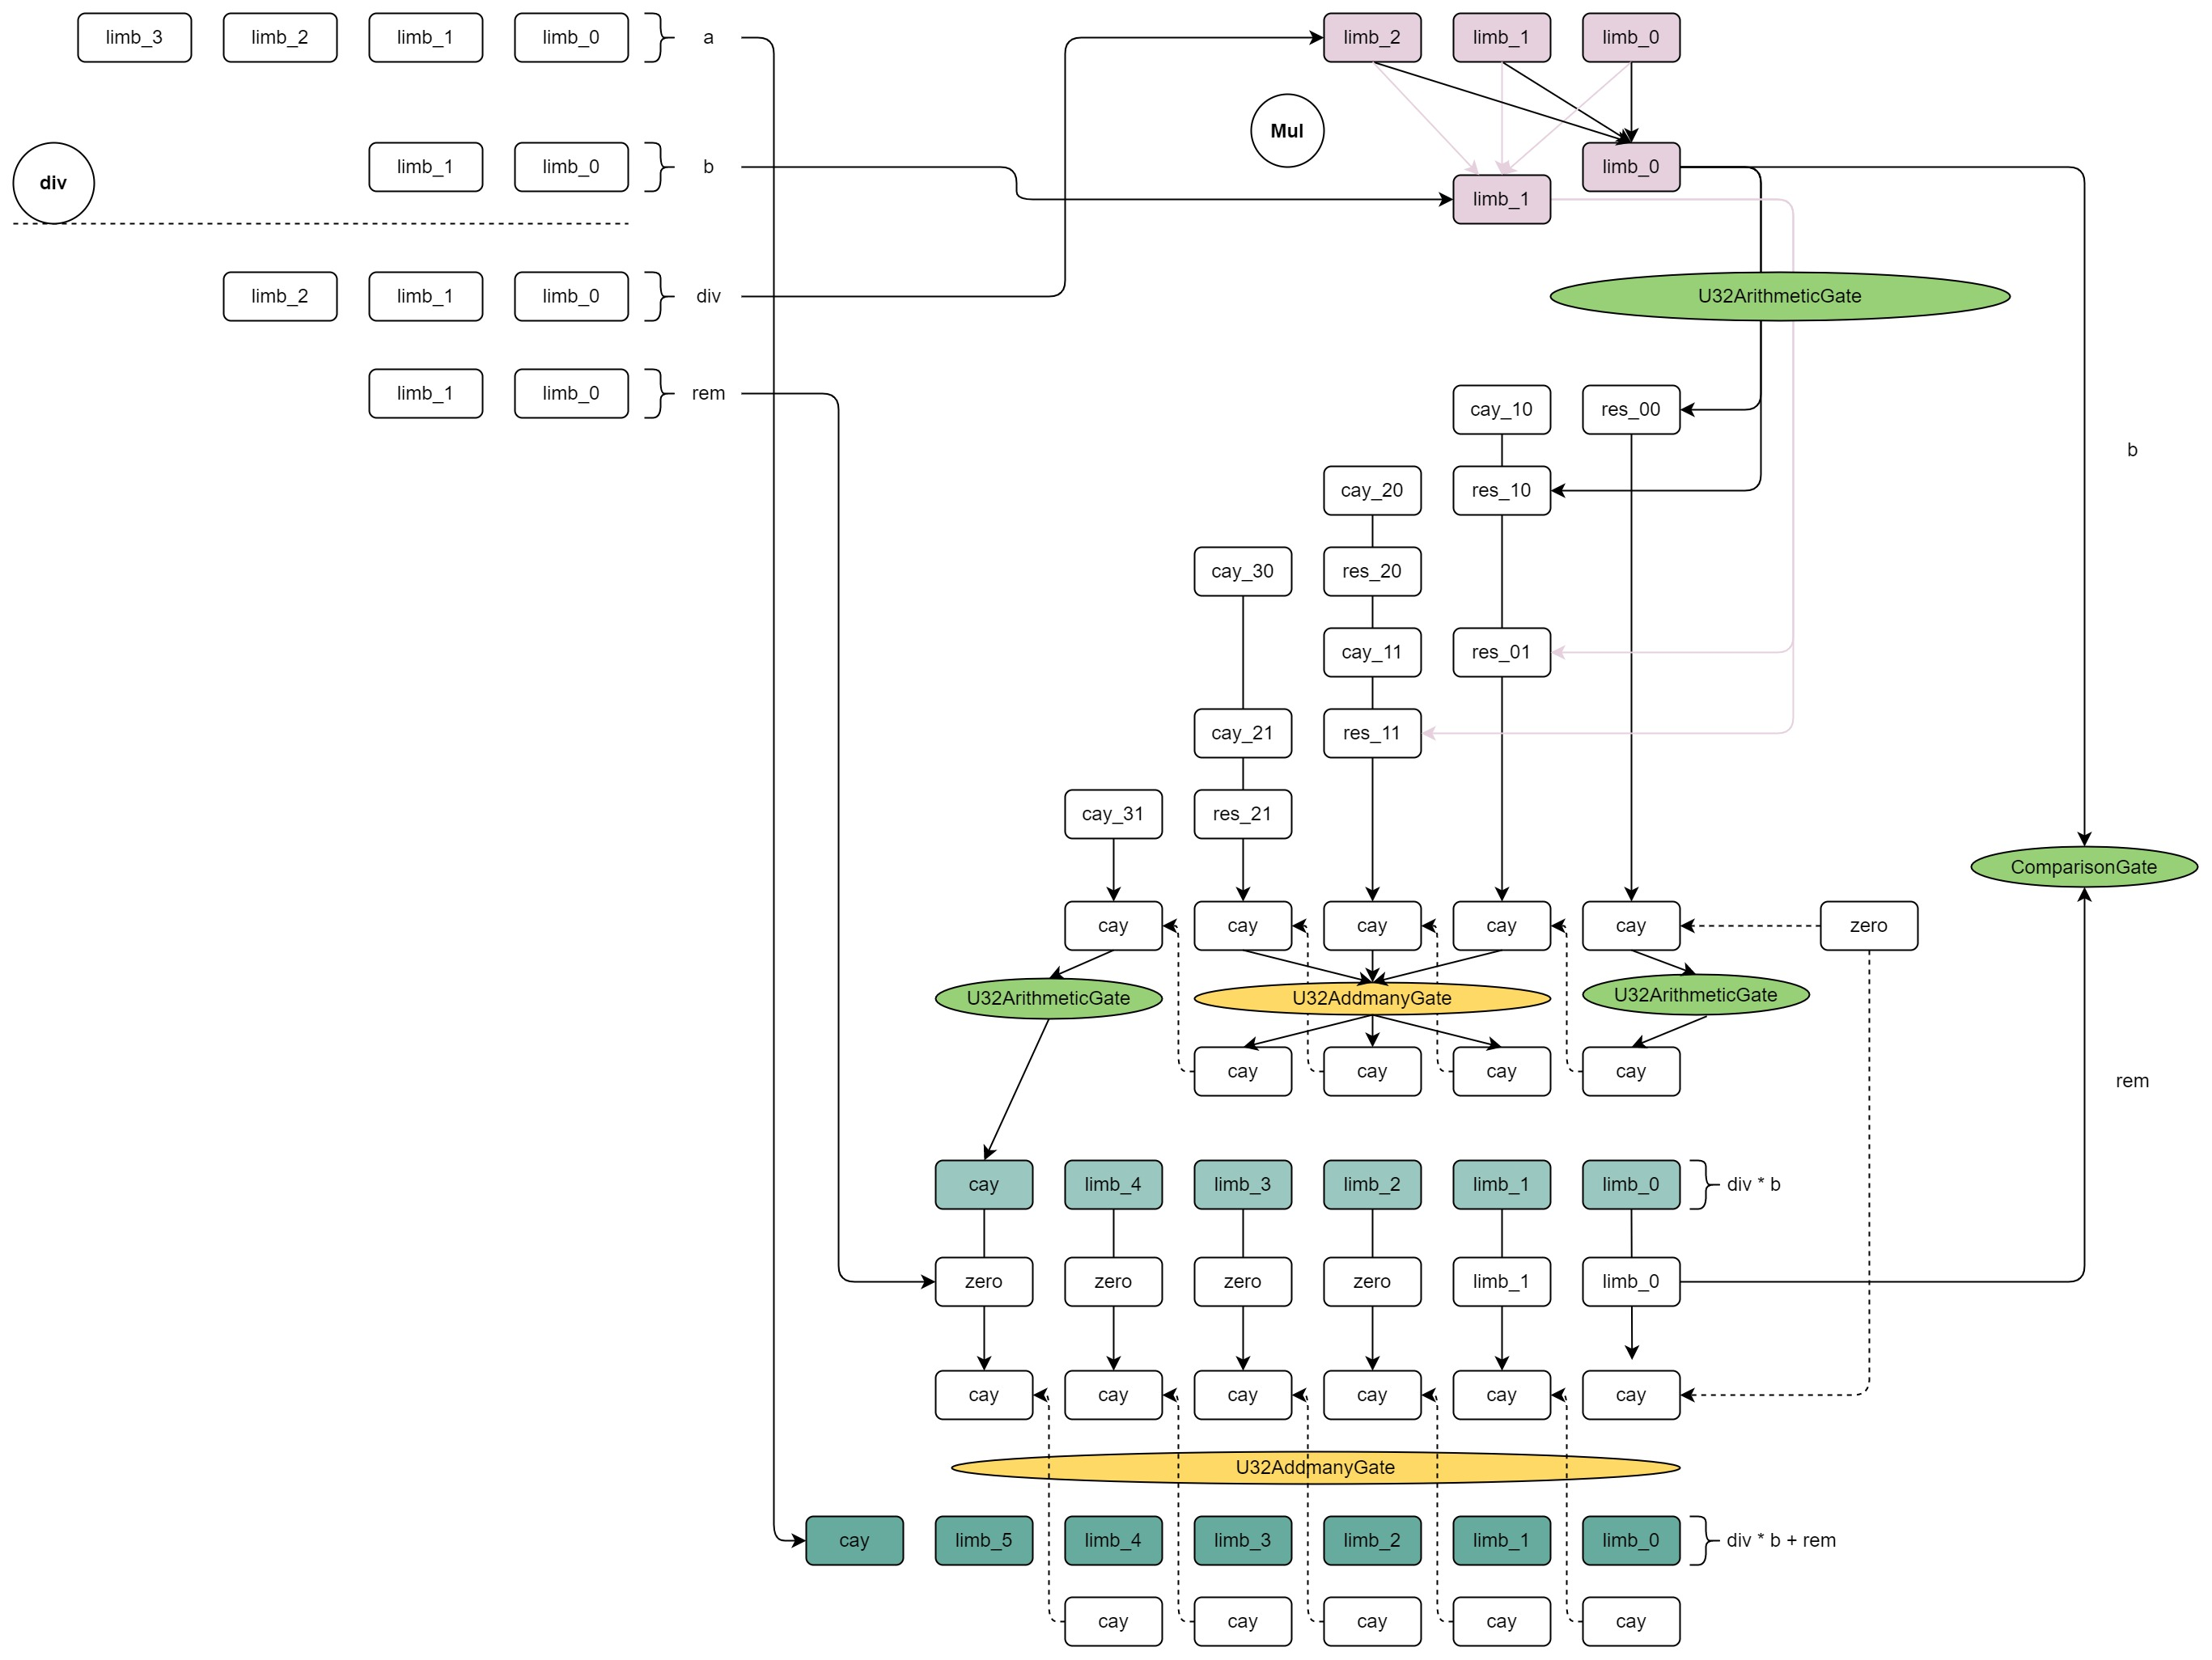
\includegraphics[width=0.8\textwidth]{biguint-div-layout.jpg}
            \caption{biguint-div layout.jpg}
            \label{fig:biguint-div-layout.jpg}
        \end{figure}
    
    \item constraints-info and costs
        \begin{itemize}
            \item Gate type num: 5(U32ArithmeticGate, U32AddManyGate(num-addends: 3), U32AddManyGate(num-addends: 4), ComparisionGate, ArithmeticGate)
            \item Gate instance num: 3 + 3 + 4 + 3 = 13 
            \item U32ArithmeticGate num: 3
            \item U32AddManyGate num: 3
            \item ComparisionGate num: 4
            \item ArithmeticGate num: 3
            \item copy-constraints: 3 * 8 + 4 + 5 + 4 + 4 * 6 + 7 + 1 + 26 + 5 = 100 
            \item max-degree: 4
        \end{itemize}

\end{enumerate}